\subsection{Konvekse mængder}
%
I forbindelse med mængder af vektorer er det vigtigt at definere \textit{konvekse mængder}.
\begin{defn}{}{konveks}
En mængde $S \subset \R^n$ er konveks, hvis $\lamda \textbf{x} + (1-\lambda )\textbf{y} \in S$ for ethvert $\textbf{x}, \textbf{y} \in S$ og ethvert $\lamda \in [0,1]$. 
\end{defn}
%
En mængde er med andre ord konveks, hvis ethvert element på en ret linje mellem to vilkårlige punkter $x$ og $y$ i mængden også tilhører mængden. På figur \ref{asdf} ses eksempler på konvekse og ikke-konvekse mængder. 

\begin{figure}[h!]
  \centering
  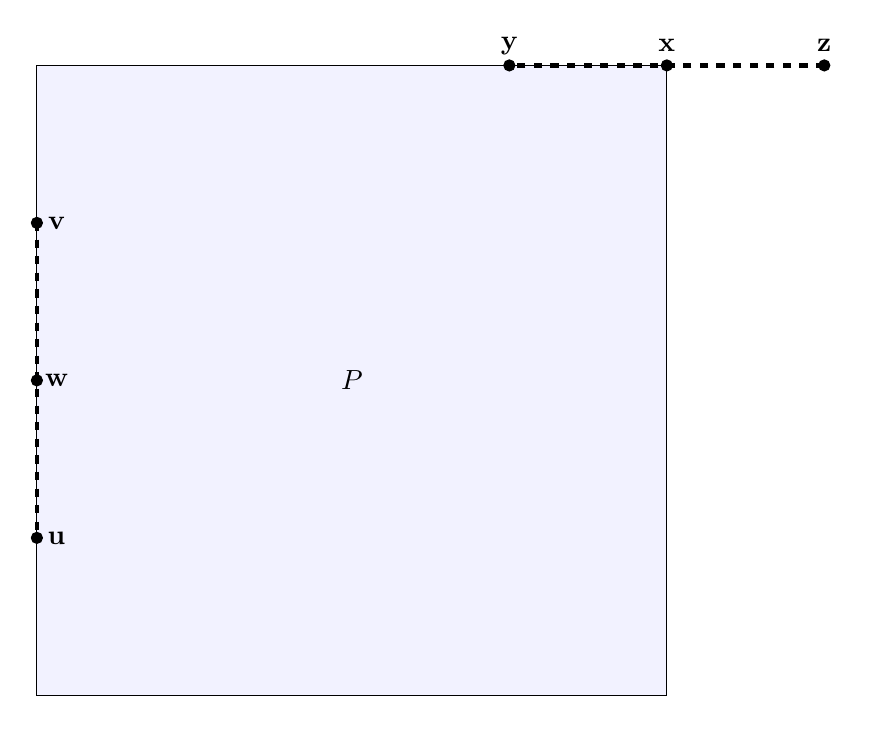
\begin{tikzpicture}
    \tikzset{punkt/.style={point, draw=black}}
    
    
%Punkter

	\node at (4,4)	(1){};
	\node at (-4,4)	(4){};
	\node at (4,-4)	(2){};
	\node at (-4,-4) (3){};


	\filldraw[black, fill=blue!5] (2) rectangle (4);
	\node at (0,0) (P){$P$};
	
	\filldraw [black] (2,4) circle (2pt);
	\filldraw [black] (4,4) circle (2pt);
	\filldraw [black] (6,4) circle (2pt);
	\filldraw [black] (-4,2) circle (2pt);
	\filldraw [black] (-4,0) circle (2pt);
	\filldraw [black] (-4,-2) circle (2pt);	
	\node at (2,4.25)	 (y){$\textbf{y}$};
	\node at (4,4.25)	 (x){$\textbf{x}$};
	\node at (6,4.25)	 (z){$\textbf{z}$};
	\node at (-3.75,2)  (v){$\textbf{v}$};
	\node at (-3.75,0)	 (w){$\textbf{w}$};
	\node at (-3.75,-2) (u){$\textbf{u}$};


	\draw[-, dashed,black,ultra thick] (6,4) -- (2,4);
	\draw[-, dashed,black,ultra thick] (-4,2) -- (-4,-2);

  \end{tikzpicture}
  \caption{En afgrænset polytop $P$ hvor $\textbf{x}$ er et ekstramapunkt da der ikke findes vektorer $\textbf{y}$ og $\textbf{z}$ sådan at $\mathbf{x}=\lambda\mathbf{y}+(1-\lambda)z$. $\textbf{w}$ er i modsætning ikke et ekstremapunkt da der findes $\textbf{v}$ og $\textbf{u}$ sådan at $\mathbf{w}=\lambda\mathbf{v}+(1-\lambda)u$.}
  \label{fig:ekstrema}
\end{figure}